\documentclass[12pt]{article}
 
\usepackage[margin=1in]{geometry} 
\usepackage{amsmath,amsthm,amssymb,outlines}
\usepackage{graphicx}
\usepackage{tikzsymbols}

\newcommand{\Sp}{\mathbb{S}}
\newenvironment{statement}[2][Statement]{\begin{trivlist}
\item[\hskip \labelsep {\bfseries #1}\hskip \labelsep {\bfseries #2.}]}{\end{trivlist}}

\begin{document}
 
\title{TDA HW1} 
\author{Dahlen Elstran} 
\maketitle

\begin{statement}[Problem]{1}
  Let $f: \Sp^1 \rightarrow \Sp^2$ be a continuous map which is not surjective. Prove that it is homotopic to a constant map.
\end{statement}
\begin{proof}
  If $f$ is not surjective, then there exists some $x \in \Sp^2$ such that $x \notin f(\Sp^1)$. So we can consider 
  $f(\Sp^1)$ to be $\Sp^2 \setminus \{x\}$, which is homotopy equivalent to a point:
  \par \begin{center} 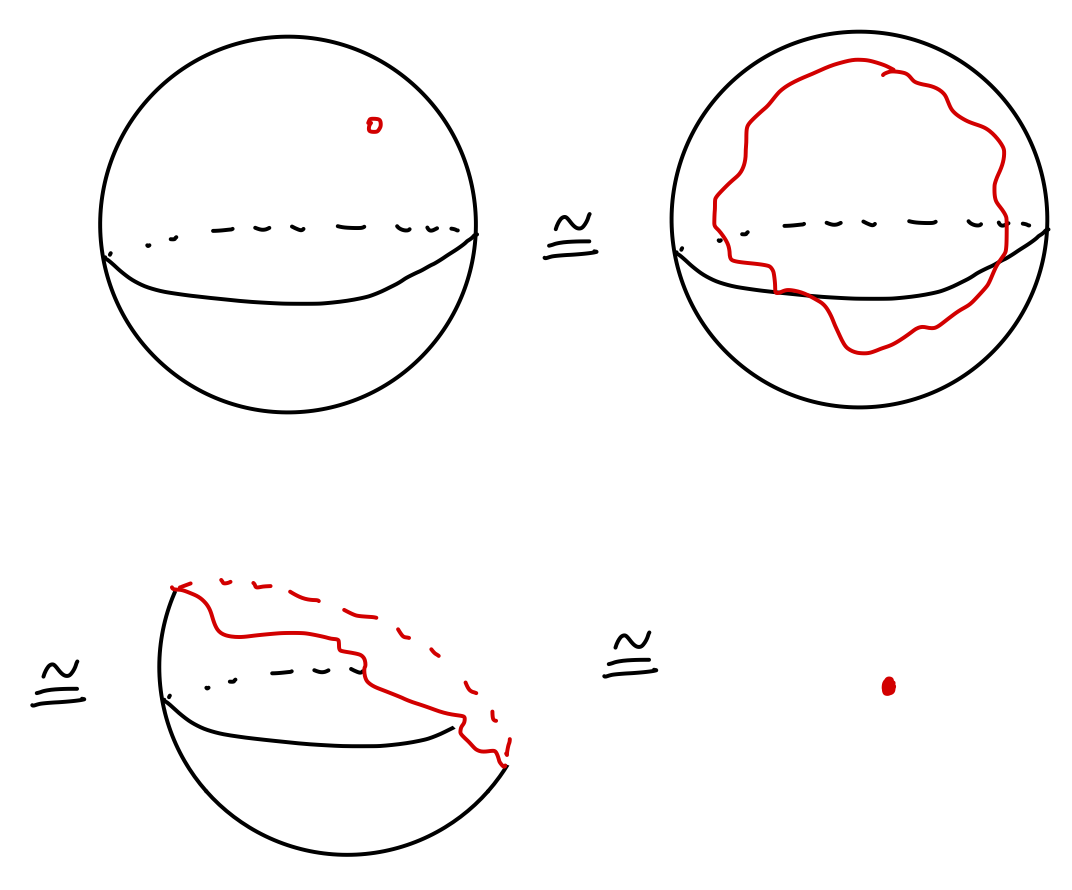
\includegraphics[scale=.2]{1-1.png} \end{center}
  Thus every map in $f(\Sp^1)$ is homotopic to a constant map. 
\end{proof}

\begin{statement}[Problem]{2}
  Let $X$ and $Y$ be two homeomorphic topological spaces. Show that if $X$ has dimension $n$, then $Y$ also has dimension $n$.
\end{statement}
\begin{proof}
   Consider a homeomorphism $f: Y \to X$, and then let $y \in Y$ with $x = f(y)$. Because $x \in X$, $x$ must have dimension 
   $n$, so that there eists an open set of $X$, call it $O$, containing $x$ with a homeomorphism $h: O \to \mathbb{R}^n$. 
   Then, we can let $O'=f^{-1}(O)$, and note that it is an open set of $Y$ containing $y$. We also know that 
   $h \circ g: O' \to \mathbb{R}^n$ is a homeomorphism, and so $Y$ has dimension $n$.
\end{proof}

\begin{statement}[Problem]{3}
Let $(G,+)$ be a group. Prove that
    $$ \forall g \in G, g+g = 0 \Rightarrow G \hspace{0.2cm} \text{is commutative}.$$
\end{statement}
\begin{proof}
  Let $g_1,g_2 \in G$, and note that $g+g=0 \iff g=-g$. Then 
  \begin{align*}
    (g_1 + g_2) + (g_1 + g_2) &=  0 \\
    g_1 + g_2 & = -(g_1 + g_2) \\
    g_1 + g_2 &= (-g_2) + (-g_1) \\
    g_1 + g_2 &= g_2 + g_1
  \end{align*}
  Thus the group is commutative.
\end{proof}

\begin{statement}[Problem]{4}
 Characterize the two surfaces depicted in Figure \ref{fig:surfaces}  in terms of genus, boundary, and orientability.

    \begin{figure}[ht]
        \centering
        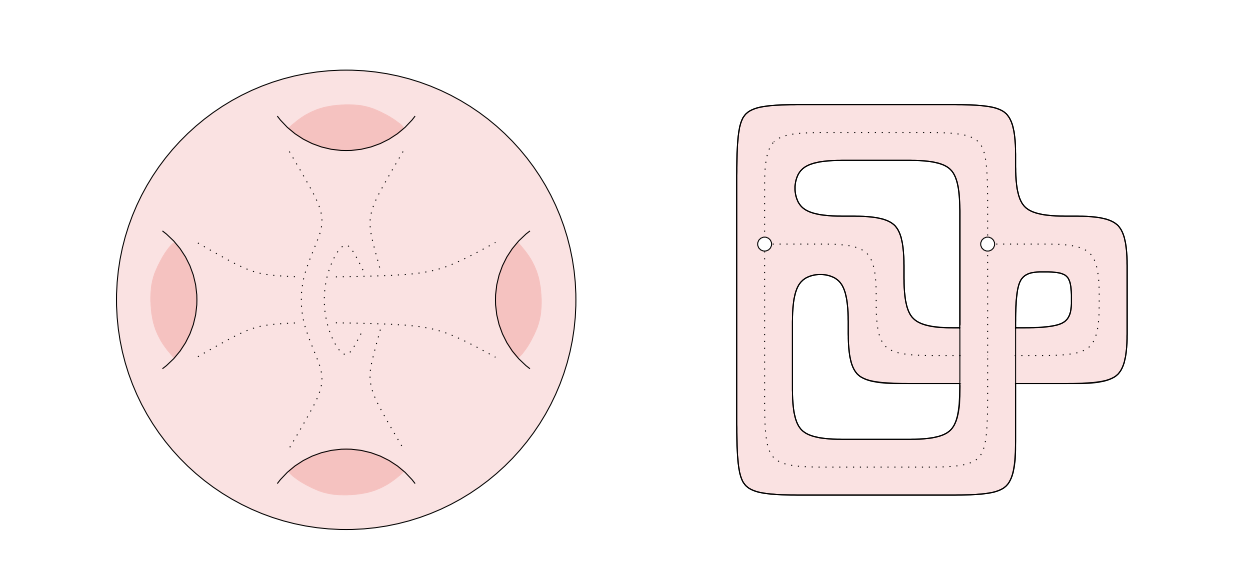
\includegraphics[width=0.5\linewidth]{surfaces.png}
        \caption{Left: a 2-manifold without boundary obtained by adding tunnels inside the sphere. Wee see four tunnel openings and one tunnel passing though a fork of the other. Right: a 2-manifold with boundary obtained by thickening a graph.}
        \label{fig:surfaces}
    \end{figure}
\end{statement}
\begin{proof}

\end{proof}

\begin{statement}[Problem]{5}
  Is every graph that can be embedded on the Mobius strip planar?
\end{statement}
\begin{proof}
  No. A counterexample would be $K_{3,3}$, which is not planar: 
  \par \begin{center} 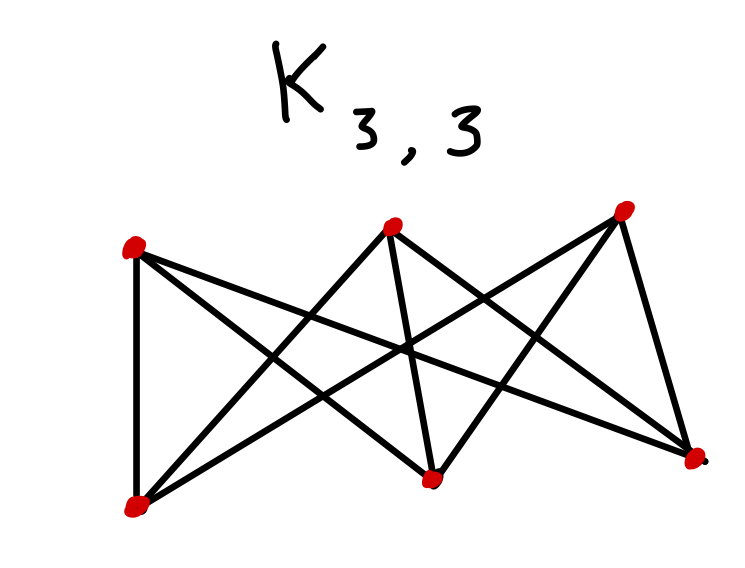
\includegraphics[scale=.2]{5-1.png} \end{center}
  However, it can be embedded on the Mobius strip.
\end{proof}

\end{document}
